%%%%%%%%%%%%%%%%%%%%%%%%%%%%%%%		CHAP 3		%%%%%%%%%%%%%%%%%%%%%%%%%%%%%%%

\chapter[Data Acquisition]{Data Acquisition system}
\label{cha:3}

Modern high energy Physics experiment's require automated procedures to collect data from detectors %
and save them in long term storage for ensuing analysis.
These routines are gathered in automated system called Data Acquisition system (DAQ), %
which typically includes three fundamental components:
\begin{enumerate}
  \item sensors, to convert physical parameters to electrical signals;
  \item signal conditioning circuitry, to convert sensor signals into a form that %
    can be converted to digital values.
  \item conversion from analog signals to digital values and subsequent storage.
\end{enumerate}
The last step is vital in that it allows data manipulation and analysis by a computer.

As far as ANNIE is concerned, the first requirement has already been discussed in section~ref: %
the experiment has multiple simultaneous data sources, i.e. %
the forward Veto, water PMTs and the MRD, as well as a blend of front-end %
electronics technologies (VME, CAMAC and custom FADCs) for ADC/TDC and waveform digitisation.
Considering this variety of devices, the whole system has also some requirements to achieve:
\begin{itemize}
  \item stability, on long acquisition runs;
  \item control all the aspect of the experiment;
  \item real time online monitoring;
  \item direct and remote user control.
\end{itemize}

Provided a solid electronic system, these tasks are thoroughly accomplished on the %
software's side, since the system is based upon the %
\emph{ToolDAQ Framework}\footnote{ToolDAQ %
  is open source and available on GitHub~[repo].}, developed %
by Dr Benjamin Richards~[ref] for the Hyper Kamiokande collaboration (HK).
The HK group has used this opportunity to undertake R\&D and testing of %
DAQ software and tools for future use in the HK experiment.
ANNIE experiment has allowed extensive testing of the flexibility of the software %
and all the above features to take place within a single deployment.

ToolDAQ is designed to incorporate the best features of other frameworks along with:
\begin{itemize}
  \item being very easy and fast to develop DAQ implementations in a very %
    modular way;
  \item Dynamic Service Discovery and Publishing; %
  \item scalable network infrastructure (provided by ZeroMQ) to allow its use on large scale experiments.
\end{itemize}

\begin{wrapfigure}{R}{0.5\textwidth}
  \centering
  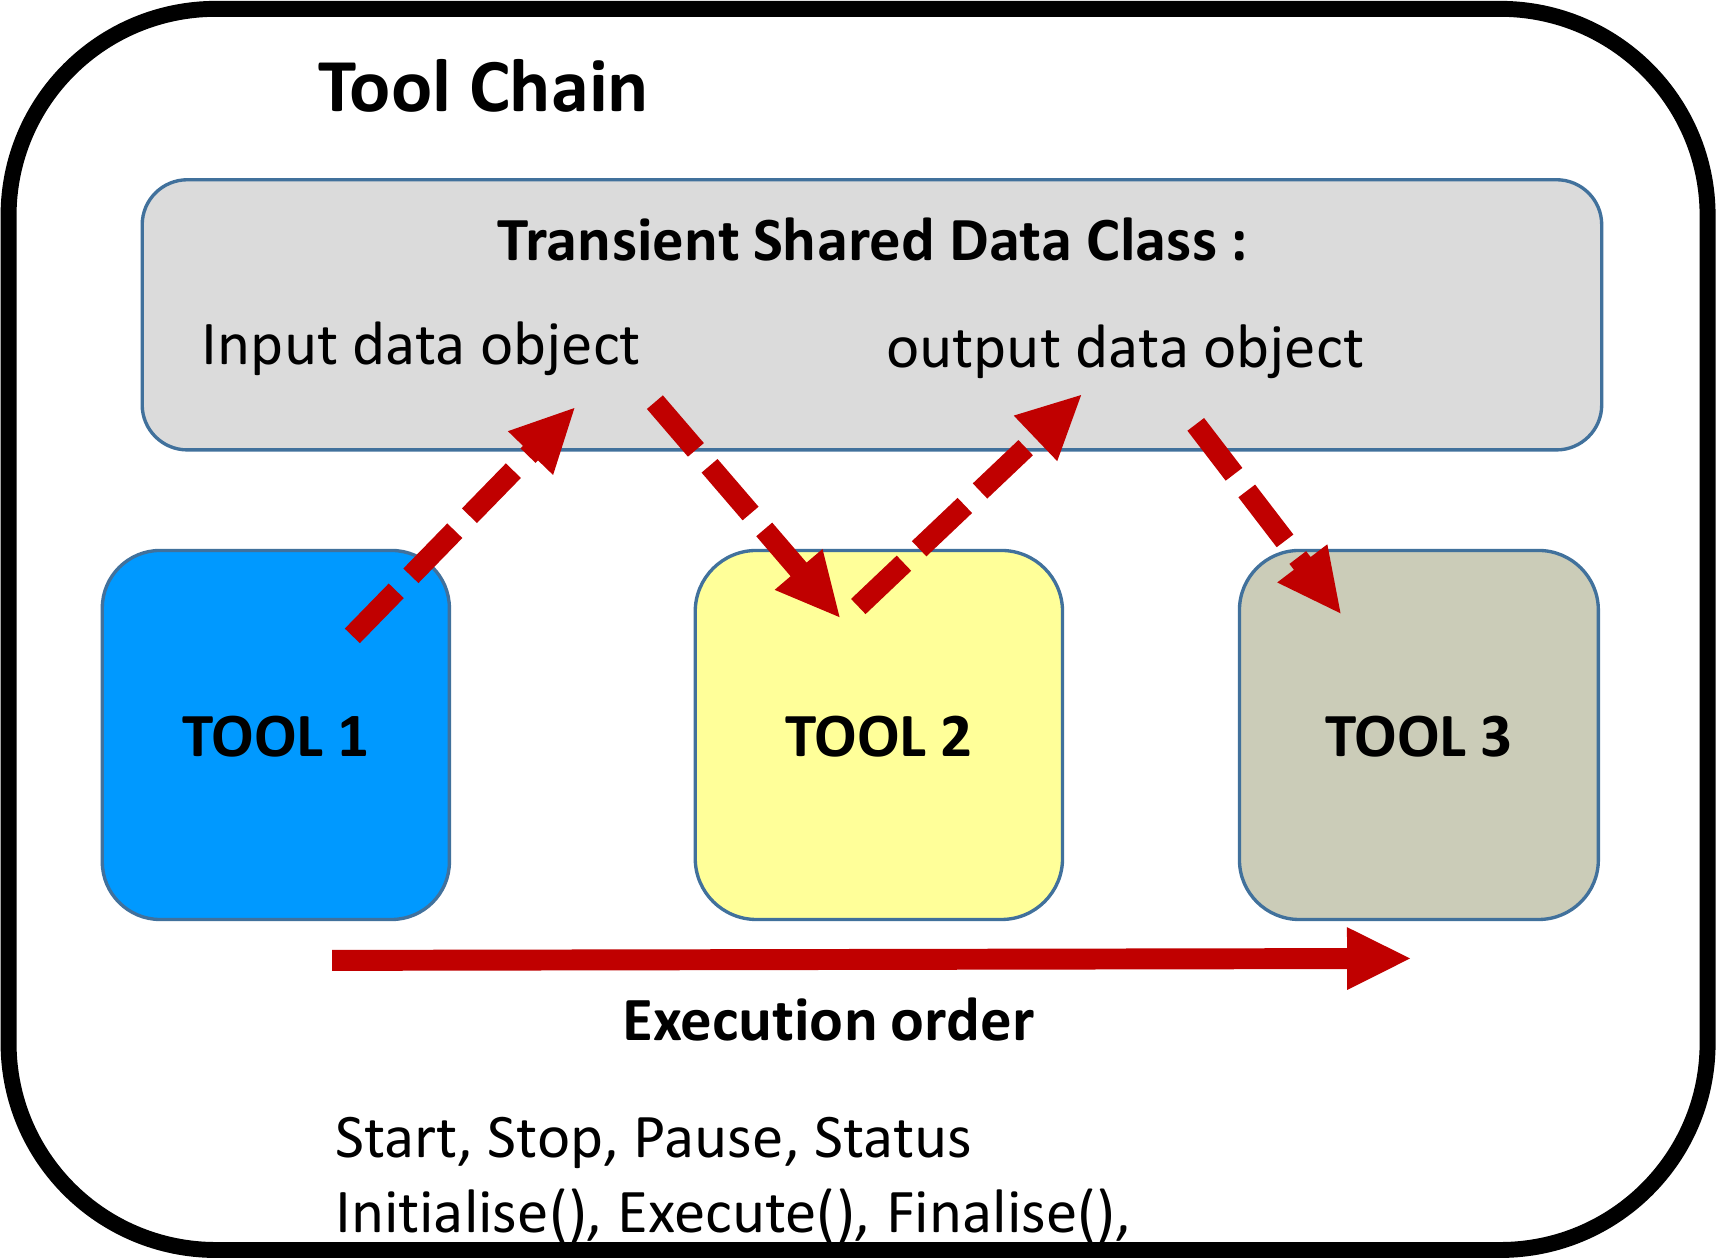
\includegraphics[scale=.13]{pics/pag4richardshkcollaboration}
  \caption{Schematic of a ToolChain.}
  \label{fig:toolchain}
\end{wrapfigure}

The main executable relies on user-defined modular classes, called \emph{Tools}, which 
present three chief functions, \emph{Initialise}, \emph{Execute}, and \emph{Finalise}.
The Tools can be daisy-chained to a \emph{ToolChain} and then handled sequentially by the process %
whenever one of those functions is called.
A ToolChain also manages the more complicated aspects of the DAQ system, %
like the remote control, the service discovery, and the status of the contained Tools.
Parameters, data and other variables are passed between Tools by an editable shared data class.
Each tool is allowed to read, update, and modify it, due to it is owned by the ToolChain.
The bare structure is sketched in Fig.~\ref{fig:toolchain}.

In the following sections, the whole DAQ structure is analysed as it currently is.
It is composed of three parallel ToolChains: the Main DAQ Chain, the VME Chain, and %
the CAMAC/MRD Chain.
The latter hasn't been implemented in the Main DAQ system yet, which is composed by the %
first two Chains only.
At the moment the MRD Chain/DAQ is employed as a standalone DAQ, working in parallel %
with the Main DAQ, on a different machine with resulting difficulties.
Future integration of the two DAQ in the same machine are also discussed.

\section{Main DAQ Chain and VME Chain}
\label{sec:3.1}

\subsection{Hardware}

The primary readout for ANNIE Phase I is provided by a VME-based system developed for the KOTO %
experiment\footnote{The KOTO experiment at J-PARC, Japan, aims at observing the rare kaon decay %
  $K_L\rightarrow \pi^0 \bar{\nu} \nu$ to search for new physics beyond the standard model that %
  breaks the CP symmetry. The experiment, with a new beam line and new detector components, is %
  underway and the first run was performed in May 2013.} %
by University of Chicago.
The \emph{VMEbus} is a computer architecture, where ``VME'' stands for VERSA Module Eurocard.
It was originally developed by the Motorola, Mostek, and Signetics group, but later was widely %
used for many applications and eventually standardised by the IEC as ANSI/IEEE 1014-1987.
This bus is widely used in High Energy Physics due to the fact that it is of public domain and %
its data transfer speed is quite fast: for instance the latest manifestation, %
the VME320/2eSST protocol, can double the theoretical bandwidth of VME to 320MB/s.
cite[http://www.vita.com/VME320-2eSST-Protocol].

The system consists of two types of VME module:
\begin{itemize}
  \item 4-channel 500~MHz sampling pipeline 14 bit custom FADC cards, which primarily record %
    the traces from the PMTs in the ANNIE water volume.
  \item Master Trigger (MT) cards which distribute the 125~MHz clock, synchronises the FADC %
    cards, provides the trigger, and provides a busy signal.
\end{itemize}

The leading edge of photomultiplier signal is too fast for an 8-ns sampling.
To avoid dead time and allow the 500~MHz sampling, the output signals from the detectors %
are stored in 8000 samples pipelines inside Field Programmable Gate Arrays (FPGAs) until %
a trigger decision is made.
The three levels trigger system uses the waveform information with increased %
sophistication at each level.
Each MT card can address 8 FADC cards, but can be daisy-chained or arrange hierarchically to %
address more total cards.
Given the 16 FADC cards of the ANNIE readout, 3 MT cards are used: %
one Level-0 card distributes the clock between two Level-1 MT cards, each addressing 8 FADCs.

The Muon Range Detector and the Forward Veto nominally rely on the same FADC system as %
the PMTs in the water volume for the first runs.
The signals coming from the paddles are combined through an analog OR and sent to a %
few spare FADC channels on the KOTO boards. 

\textcolor{blue}{
The instrumenting the ANNIE water volume are operated at positive HV with a %
single cable for both power and signal.
Splitter boxes will be necessary to separate the PMT signal and the HV.
ANNIE uses a CAEN system to provide the positive and negative high voltages necessary for operation. 
A stock of 6 A734P cards suffices to power the 62 large PMTs in the water volume %
and the 26 positive HV PMTs in the MRD.
26 negative HV channels are also needed for the Forward Veto and another 52 channels to power %
at least two layers of the MRD.
}

For storage limitations, a downsampling to 125~MHz was established.
The resolution of 8~ns suffices the needs of the R\&D stage of Phase I.
An 80~$\mu$s long time window wash chosen, therefore with this resolution, four data sets can be %
hold in the 40000 samples buffer.
Each set corresponds to a spill from the beam.

\subsection{Software}

The data from the water PMTs and the logical sum from the Veto and MRD are acquired by the Main DAQ, %
which hinges upon two strictly complementary ToolChains: the Main Chain and the VME Chain.
The Main Chain is the primary ToolChain of the DAQ system, which communicates with the other two %
processes.

The Chain's tools are depicted in Fig.~\ref{fig:anniedaq} and they are the following:

\begin{center}
  \small
  \begin{tabular}{cc}
    \toprule
    \textbf{Main DAQ}	& \textbf{VME}		\\
    \midrule
    Input variables 		&   \\
    PostSQL 			& VME Trigger Send   \\
    Trigger			& Board Reader	\\
    Network Receive Data	& Network Send Data	\\
    Monitor			& 	\\
    Data Recorder		& 	\\
    \bottomrule
  \end{tabular}
\end{center}

The \emph{Input variables} tool loads some initialisation parameters and the specification of %
the current \emph{run}, i.e. data taking session.
Three typologies of run are available and are sent to the VME CPU: a test run, an LED run for PMTs %
calibration, a pedestal run, and a beam run.
The triggering of the digitisers is influenced by changing the kind of the run.
For instance, a beam run is triggered by the RWM, while an LED run is triggered by the LED pulser.
The \emph{PostSQL} tool updates an SQL database of the DAQ, where all the information about %
the run, such as the number of events, the start and the stop time, and others, are saved.
Proper data logging is a fundamental step, especially for Phase I: both the experiment and the DAQ %
are frequently revised and \textcolor{red}{knowing which run is which is pretty cool.}
\emph{Trigger} tool blocks the Chain, awaiting and sending a trigger query from the VME.
When the VME replies, the Chain is run back again.
As explained, four 10000samples data sets are collected from the VME cards, which equates to %
four consecutive spills from the beam.
The \emph{Network receive data} tool handles the data transfer via ZeroMQ %
messaging\footnote{\emph{ZeroMQ} %
  is a high-performance asynchronous messaging library, aimed at use in distributed applications.
  The API provides \emph{sockets}, each of which can represent a many-to-many connection %
  between endpoints, operating with a message-wise granularity.
  ZeroMQ is developed by a large community of contributors and distributed under the LGPL license.
  http://zeromq.org/} %
between the main chain and the VME one.
Like most of the HEP experiments, even ANNIE requires real-time monitoring so as to check whether %
the DAQ system works flawlessly.
This is achieved by the \emph{Monitor} tool, which updates a dedicated web-page with %
random plots of data collected.
The last too, \emph{Data recorder}, saves acquired data into a ROOT trees structure.
Each entry corresponds to a spill, i.e. a trigger in the VME cards, and holds a 10000 long float %
array containing the digitised time window.
In the same entry, other values are stored (PMT number, spatial position, channel, card etc..).
Among these, the TimeStamp is fetched from the ADC cards.

\begin{figure}[]
  \centering
  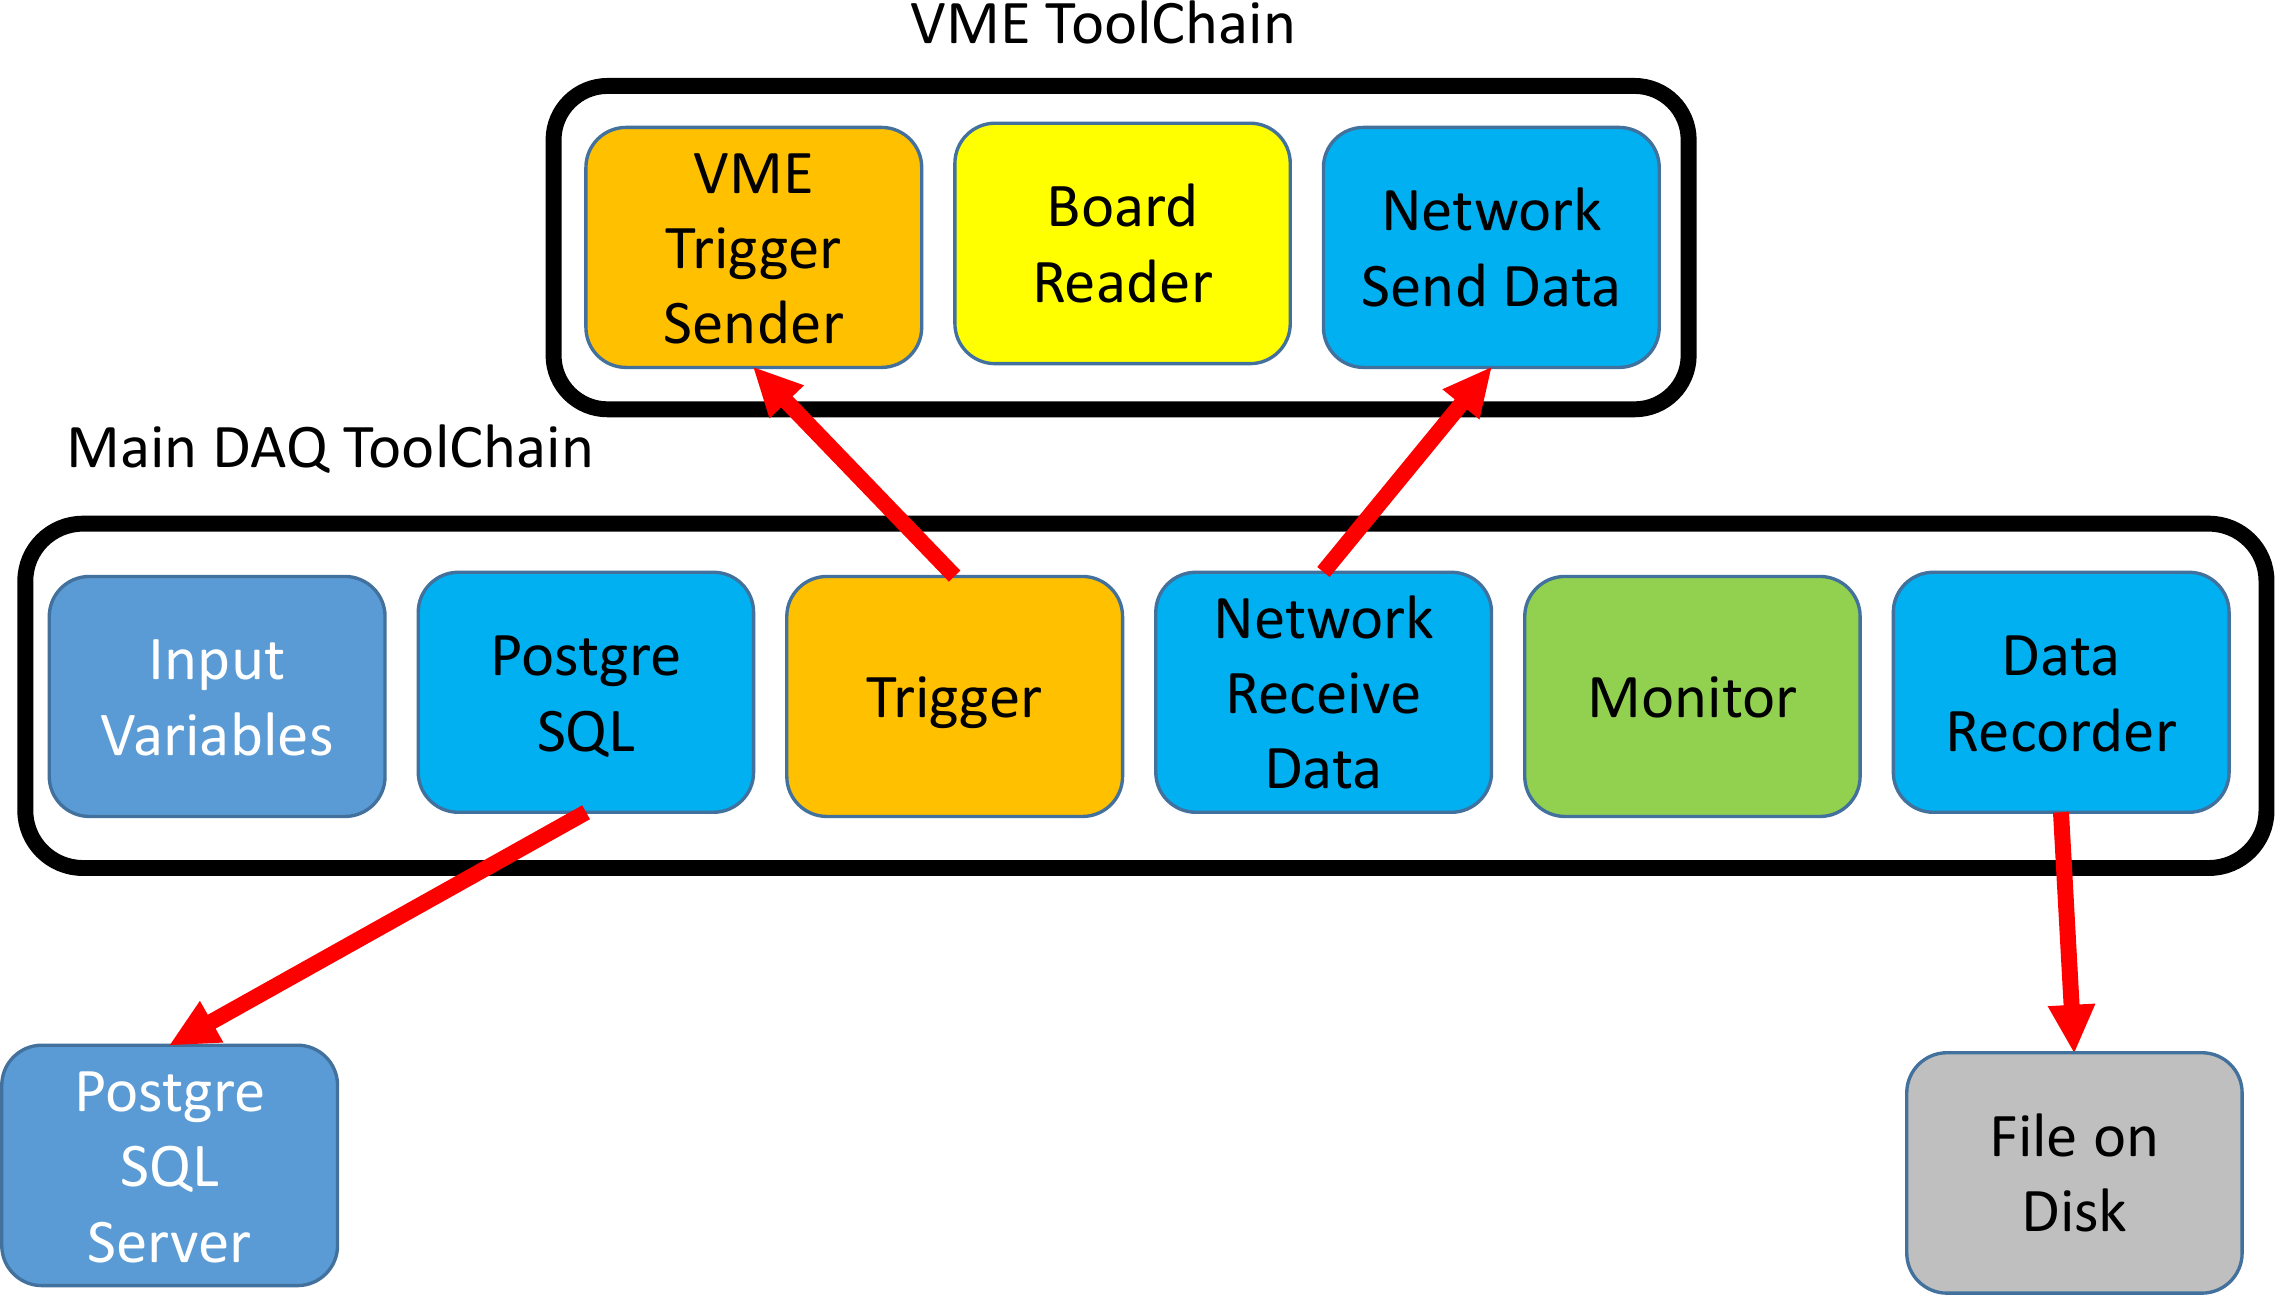
\includegraphics[scale=0.20]{pics/pag2richardshkmeeting}
  \caption{ANNIE's current main DAQ makes use of two parallel tool chains.}
  \label{fig:anniedaq}
\end{figure}

A ToolChain has also been developed to address the VME crates.
As illustrated in Fig.~\ref{fig:anniedaq}, the Tools contained in this Chains are
\begin{enumerate}
  \item Trigger sender;
  \item Board reader;
  \item Network send data;
\end{enumerate}

\emph{Trigger sender} is given by RWM.
Talk about downsampling and buffer sizes.
\emph{Board reader} gets data from ADC, ready to be sent.
\emph{Network} send data over network.
\textcolor{green}{Ask Ben, he should know.}

\textcolor{red}{Not finished yet. Have to talk about output format too.}

\section{MRD Chain}
\label{sec:3.2}

\subsection{Hardware}

As explained in Sec.~\ref{sec:3.2}[edit to section of VME], the signal from the FACC %
and two layers of the MRD are logically summed and read by the VME digitisers.
The PMTs of these two detectors are meant to be read individually by both Time to Digital %
Converters (TDC) and ADCs in future stages of the experiment.
A third ToolChain has been developed to collect data from both the VETO and %
the MRD's second and third layers.
CAMAC electronic modules are employed for these two detectors: LeCroy 3377 modules for the time %
digitisation, while LeCroy 4300B for analog conversion.

\emph{Computer-Aided Measurement And Control} (CAMAC) is a bus and modular-crate electronic %
standard for data acquisition and control used mainly in nuclear and particle physics experiments %
and in industry.
The bus allows data exchange between plug-in modules and a crate controller, %
which then interfaces to a CPU or to a VME-CAMAC interface.
The standard was originally defined by the ESONE Committee as standard EUR-4100 in 1972.

The LeCroy Model 3377 is a 32-channel time-to-digital converter (TDC) and %
optimised with a low conversion time and a high speed readout of 100~ns/word.
With 10-bit words, the longest time window achievable is \np{4088.0}~ns, using a resolution %
of 4.0~ns.
A delayed signal from the RWM acts as a ``common start'' for the TDC cards and %
each internal counter is individually stopped by hit signals.
The channels are fed with the discriminated PMT signals of the VETO and of the second %
and the third layer of the MRD.

The LeCroy Model 4300B FERA contains 16 independent 11bit charge-to-digital converters.
An 8-bit register and a memory containing the individual pedestal values to be subtracted from %
each ADC are also available.
These converters haven't been installed in the electronic chain yet.
Nevertheless the software interface has been developed anyway.

All the cards are addressed via the Weiner CCUSB controller module. 
The CCUSB is a full-featured CAMAC Crate controller with integrated high speed USB-2 %
interface.
For fast data acquisition applications the CCUSB has a built-in command list sequencer, called %
\emph{command stack} with data buffering in a 22kB size FIFO.
A XILINX Spartan 3 family FPGA performs all CCUSB logic and functions. 
The MRD rate has been found to be quite low in this early stage (event rate \np{0.20}~Hz), since %
only two layers are used.
For these reasons, the command stack is not employed ,since the USB connection is fast enough %
to address all the active cards. 


\textcolor{red}{More on this?}


\subsection{Software}

A separate MRD DAQ has been created within the ToolDAQ Framework in order to acquire the MRD %
and the forward Veto data.
These two detectors rely on the CAMAC electronics for front-end read out of the PMTs %
signals and the USB controller vendor provides a C++ class to interface the controller with the %
computer.

Some C++ classes were developed with the purpose of handling more easily the modules.
A base class takes care of opening the USB connection for the CCUSB controller and storing %
information on the cards, such as the Slot number.
It also allows the configuration of the command stack, i.e. the CAMAC command sequencer.
Two derived classes implement wrapper functions to deliver CAMAC commands via the %
NAF addressing\footnote{Module addressing is achieved knowing the slot \textbf{N}umber, %
the sub\textbf{A}ddress, and the \textbf{F}unction code.}.

The MRD's ToolChain employs the CAMAC classes to interface with the controller and the cards.
As illustrated in Fig.~\ref{fig:anniedaq}, the Tools contained in the Chain are:
\textcolor{red}{picure of mrd chain alone.}

\begin{center}
  \small
  \begin{tabular}{c}
    \toprule
    \textbf{MRD}	\\
    \midrule
    Trigger	\\
    LeCroy 	\\
    Root output	\\
    \bottomrule
  \end{tabular}
\end{center}

The \emph{Trigger} tool reads the FIFO of a specified card: if it is not empty, then all %
cards presenting data are read and other tools are executed.
Currently, a hit signal is generated in each TDCs by delaying the common start %
signal of $\sim 1~\mu$s, such that the FIFOs are never empty in coincidence with the beam's spills.
Three triggering behaviours are supported: external trigger, software trigger with %
random card access, and software trigger with card test function.

The \emph{LeCroy} tool is meant to work for both the TDCs and ADCs cards.
If only either TDCs or ADCs are employed, then only one tool should be added in the \emph{ToolChain}.
Otherwise, if both are used, then two \emph{LeCroy} tools are required.
Given that the ADCs haven't been installed in the crates yet, only one tool is %
needed for the TDCs.
Nevertheless the charge converters have been tested, as well.

The last tool fills a ROOT tree and save it to file.
The tree has the following branches:
\begin{center}
\begin{varwidth}{\textwidth}
\begin{itemize}
  \item[\bfseries Trigger :] incremental number of the trigger;
  \item[\bfseries OutNumber :] number of channels read;
  \item[\bfseries Type :] string telling whether the data refer to TDC or to ADC;
  \item[\bfseries Value :] actual value retrieved from the card.
  \item[\bfseries Slot :] slot number of the card;
  \item[\bfseries Channel :] channel of the card from which the value was retrieved;
  \item[\bfseries TimeStamp :] UNIX time stamp of the entry, since epoch, in ms.
\end{itemize}
\end{varwidth}
\end{center}

The MRD Chain runs in a different PC than the Main DAQ and the ToolChain %
is executed at a different speed, for it is a standalone process.
For this reason, a method has been realised to correlate the events between the two DAQs.
Timestamps were designated for this fundamental task: both DAQs assign UNIX time to each event, since %
the clocks are synchronised to the same NTP server, which uses GPS time sources.
With the help of the Fermilab spill database [ref here], the events from the two DAQs can be related %
to each other.

However, a time variable drift in the MRD TimeStamps has been found, likely due to imprecise %
synchronisation with the NTP server (accuracy given to 30~ms). 
A post-processor has been written to fix the TimeStamps, identifing time patterns in the %
spill spectrum and comparing them to the database information.

\textcolor{blue}{picture of spill sync would be nice.}

\textcolor{red}{
CAMAC interface
Performances
Synchronisation with main DAQ
Post-processing
Downsampling
Memory issues
}

\section{Future improvement}
\label{sec:3.3}
{
\color{red}
Downsampling -> was it worth it?
Zero suppression is cooler for memory issues, takes a lot of memory.

Integration between Chains, using timestamps now and database.
This technique is ok, but the chains must be implement end better each other.

One solution could be to create a tool to govern the MRD chain, as in Fig.~\ref{fig:daqcomplete}
}

The final version of the DAQ system needs a full integration of the Main Chain with the %
CAMAC one.
A possible solution is depicted in Fig.~\ref{fig:daqcomplete}.
A new tool could be employed to embody a simplified verion of the MRD ToolChain, rather than %
run it in a parallel process.
The MRD Chain is quite light and fast in execution, so it should not %
significantly slow down the Main DAQ.
In this way, the TimeStamp synchronisation technique is not required anymore because all the %
acquisitions are done by the same CPU, hence at the same time.
As far as the output files are concerned, the ROOT trees could be merged into a single ROOT file %
triggering the record tools with ZeroMQ communication.
Final reconstruction of PMTs data and MRDs could be done in a post-processing stage.

\begin{figure}[]
  \centering
  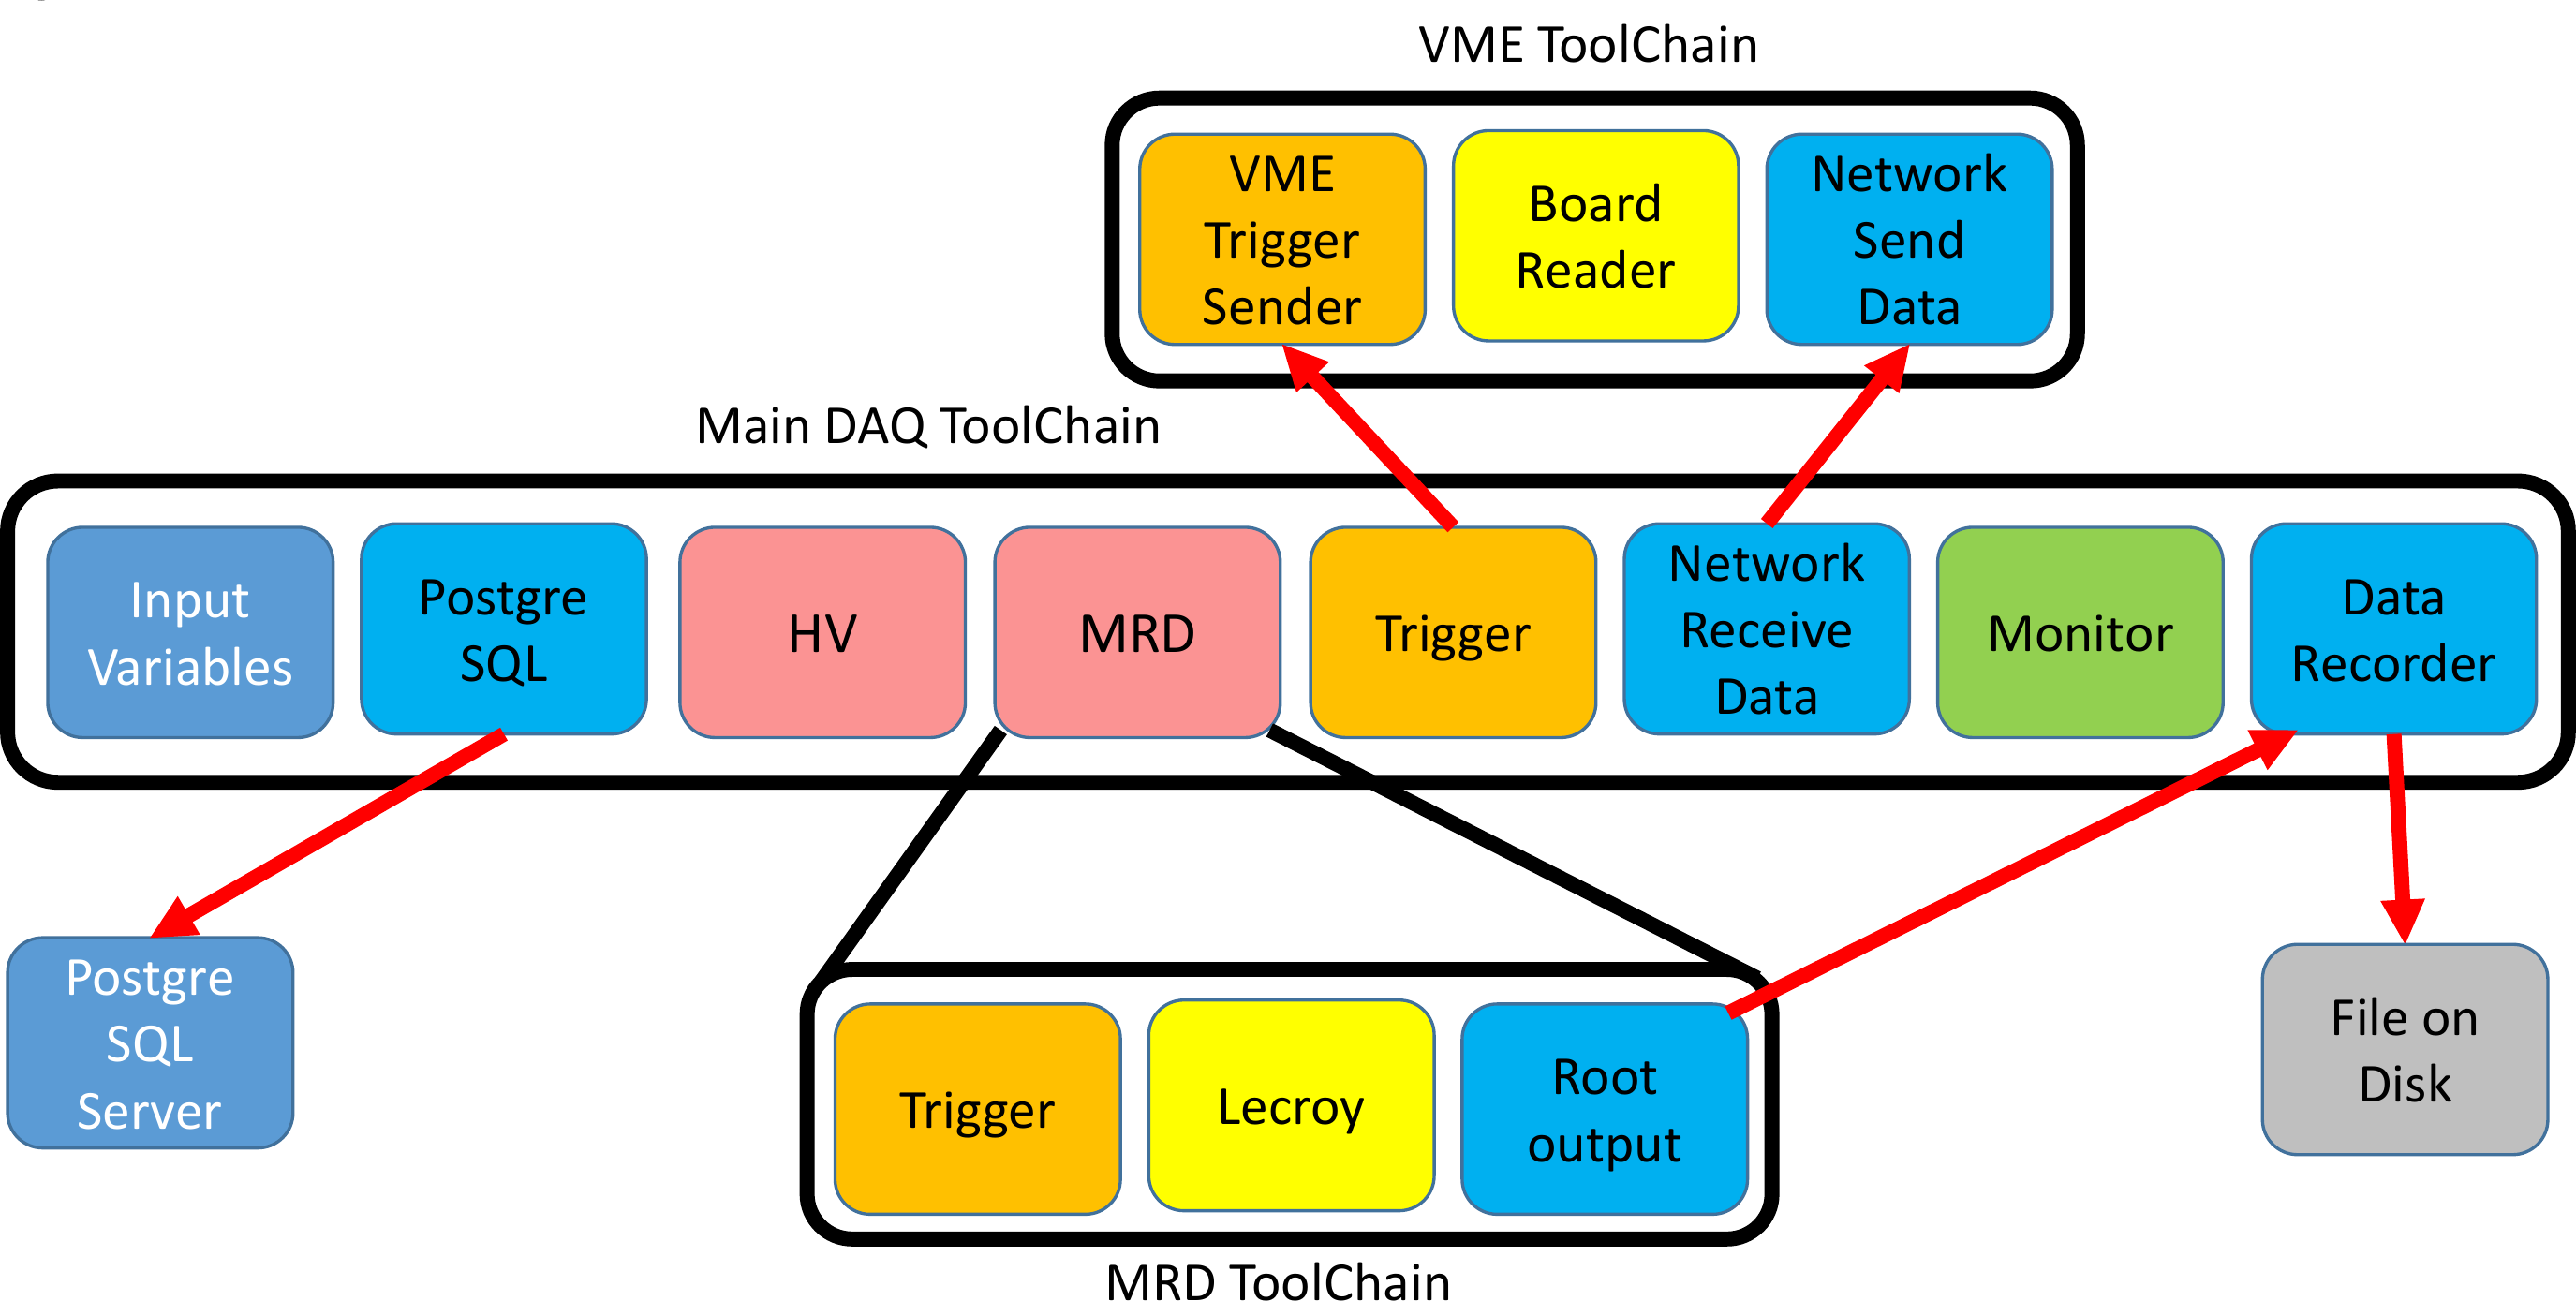
\includegraphics[scale=0.17]{pics/pag5richardshkmeeting}
  \caption{Final version of ANNIE's DAQ, with all the Chains integrated.}
  \label{fig:daqcomplete}
\end{figure}

In view of the next phases of the experiment, an other DAQ-related issue is the memory storage.
During early test runs, the digitiser would sample at a frequency of 500~MHz, but it has been %
promptly downgraded to 15~MHz because of lack of long term memory storage.
Noise is mostly shown in the 80~$\mu$s time window and the effective information is scarce.
Considering that an high time resolution is pointless in the R\&D stage of the experiment, the %
downgrade was established.
Next phases would employ zero suppression method, which will definitely overcome storage needs.
The preliminary data analysis undertaken can back up this decision, as explained in section~[ref].
